\documentclass[11pt,border=5pt]{standalone}
\usepackage{fontspec}
\setmainfont{cmunrm.otf}[BoldFont=cmunbx.otf,ItalicFont=cmunti.otf,BoldItalicFont=cmunbi.otf]
\usepackage{amsmath}
\usepackage{unicode-math}
\setmathfont{NewCMMath-Regular.otf}
\usepackage{tikz}
\usetikzlibrary{arrows.meta,patterns,angles,quotes}
\begin{document}
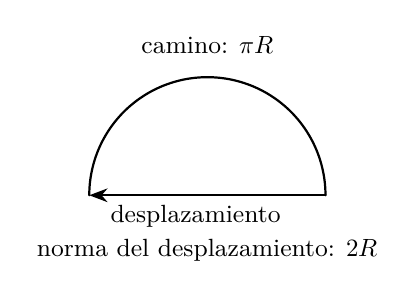
\begin{tikzpicture}[>=Stealth,font=\small,line cap=round,line join=round]
\draw[thick] plot coordinates {(1.50000,0.00000) (1.49949,0.03927) (1.49794,0.07850) (1.49538,0.11769) (1.49178,0.15679) (1.48717,0.19579) (1.48153,0.23465) (1.47488,0.27335) (1.46722,0.31187) (1.45855,0.35017) (1.44889,0.38823) (1.43823,0.42602) (1.42658,0.46353) (1.41396,0.50071) (1.40037,0.53755) (1.38582,0.57403) (1.37032,0.61010) (1.35388,0.64577) (1.33651,0.68099) (1.31823,0.71574) (1.29904,0.75000) (1.27896,0.78375) (1.25801,0.81696) (1.23619,0.84961) (1.21353,0.88168) (1.19003,0.91314) (1.16572,0.94398) (1.14061,0.97417) (1.11472,1.00370) (1.08806,1.03253) (1.06066,1.06066) (1.03253,1.08806) (1.00370,1.11472) (0.97417,1.14061) (0.94398,1.16572) (0.91314,1.19003) (0.88168,1.21353) (0.84961,1.23619) (0.81696,1.25801) (0.78375,1.27896) (0.75000,1.29904) (0.71574,1.31823) (0.68099,1.33651) (0.64577,1.35388) (0.61010,1.37032) (0.57403,1.38582) (0.53755,1.40037) (0.50071,1.41396) (0.46353,1.42658) (0.42602,1.43823) (0.38823,1.44889) (0.35017,1.45855) (0.31187,1.46722) (0.27335,1.47488) (0.23465,1.48153) (0.19579,1.48717) (0.15679,1.49178) (0.11769,1.49538) (0.07850,1.49794) (0.03927,1.49949) (0.00000,1.50000) (-0.03927,1.49949) (-0.07850,1.49794) (-0.11769,1.49538) (-0.15679,1.49178) (-0.19579,1.48717) (-0.23465,1.48153) (-0.27335,1.47488) (-0.31187,1.46722) (-0.35017,1.45855) (-0.38823,1.44889) (-0.42602,1.43823) (-0.46353,1.42658) (-0.50071,1.41396) (-0.53755,1.40037) (-0.57403,1.38582) (-0.61010,1.37032) (-0.64577,1.35388) (-0.68099,1.33651) (-0.71574,1.31823) (-0.75000,1.29904) (-0.78375,1.27896) (-0.81696,1.25801) (-0.84961,1.23619) (-0.88168,1.21353) (-0.91314,1.19003) (-0.94398,1.16572) (-0.97417,1.14061) (-1.00370,1.11472) (-1.03253,1.08806) (-1.06066,1.06066) (-1.08806,1.03253) (-1.11472,1.00370) (-1.14061,0.97417) (-1.16572,0.94398) (-1.19003,0.91314) (-1.21353,0.88168) (-1.23619,0.84961) (-1.25801,0.81696) (-1.27896,0.78375) (-1.29904,0.75000) (-1.31823,0.71574) (-1.33651,0.68099) (-1.35388,0.64577) (-1.37032,0.61010) (-1.38582,0.57403) (-1.40037,0.53755) (-1.41396,0.50071) (-1.42658,0.46353) (-1.43823,0.42602) (-1.44889,0.38823) (-1.45855,0.35017) (-1.46722,0.31187) (-1.47488,0.27335) (-1.48153,0.23465) (-1.48717,0.19579) (-1.49178,0.15679) (-1.49538,0.11769) (-1.49794,0.07850) (-1.49949,0.03927) (-1.50000,0.00000)};
\draw[->,thick] (1.5,0) -- (-1.5,0) node[pos=0.55,below] {desplazamiento};
\node at (0,1.9) {camino: $\pi R$};
\node at (0,-0.7) {norma del desplazamiento: $2R$};

\end{tikzpicture}
\end{document}
